% HALI Research Presentation
% Author: Dhruv Joshi
% LaTeX Beamer Presentation with Berkeley Theme and Seahorse Color Scheme

\documentclass[aspectratio=169,12pt]{beamer}
\usetheme{Berkeley}
\usecolortheme{seahorse}

% Packages
\usepackage{tikz}
\usepackage{pgfplots}
\usepackage{booktabs}
\usepackage{algorithm}
\usepackage{algorithmic}
\usepackage{amsmath}
\usepackage{amssymb}
\usepackage{graphicx}
\usepackage{listings}
\usepackage{xcolor}

\usetikzlibrary{shapes,arrows,positioning,fit,backgrounds,calc}
\pgfplotsset{compat=1.17}

% Title Information
\title[HALI: Hierarchical Adaptive Learned Index]{HALI: Hierarchical Adaptive Learned Index}
\subtitle{A Novel Hybrid Index Structure for Dynamic Workloads}
\author[D. Joshi]{Dhruv Joshi\\ \texttt{jdhruv1503@gmail.com}}
\institute[HALI Research]{Operating Systems Course Project\\
HALI Research Initiative}
\date{\today}

% Custom colors
\definecolor{codegreen}{rgb}{0,0.6,0}
\definecolor{codegray}{rgb}{0.5,0.5,0.5}
\definecolor{codepurple}{rgb}{0.58,0,0.82}
\definecolor{backcolour}{rgb}{0.95,0.95,0.92}

\lstdefinestyle{mystyle}{
    backgroundcolor=\color{backcolour},
    commentstyle=\color{codegreen},
    keywordstyle=\color{blue},
    numberstyle=\tiny\color{codegray},
    stringstyle=\color{codepurple},
    basicstyle=\ttfamily\footnotesize,
    breakatwhitespace=false,
    breaklines=true,
    captionpos=b,
    keepspaces=true,
    numbers=left,
    numbersep=5pt,
    showspaces=false,
    showstringspaces=false,
    showtabs=false,
    tabsize=2
}
\lstset{style=mystyle}

\begin{document}

% ============================================================
% TITLE SLIDE
% ============================================================
\begin{frame}
\titlepage
\end{frame}

% ============================================================
% OUTLINE
% ============================================================
\begin{frame}{Outline}
\tableofcontents
\end{frame}

% ============================================================
% SECTION 1: INTRODUCTION
% ============================================================
\section{Introduction \& Motivation}

\begin{frame}{The Index Problem in Modern Systems}
\begin{columns}
\column{0.5\textwidth}
\textbf{Traditional Indexes}
\begin{itemize}
    \item B+Tree, Hash Table, Radix Tree
    \item \textcolor{red}{High memory overhead}
    \item Pointer chasing $\rightarrow$ cache misses
    \item But: Predictable performance
\end{itemize}

\vspace{0.5cm}

\textbf{Learned Indexes}
\begin{itemize}
    \item Use ML models instead of pointers
    \item \textcolor{green}{Low memory footprint}
    \item Few cache misses
    \item But: \textcolor{red}{Poor dynamic performance}
\end{itemize}

\column{0.5\textwidth}
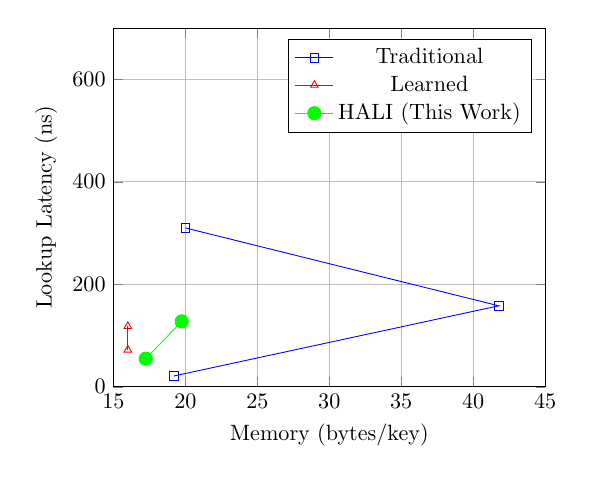
\begin{tikzpicture}[scale=0.8]
\begin{axis}[
    xlabel={Memory (bytes/key)},
    ylabel={Lookup Latency (ns)},
    xmin=15, xmax=45,
    ymin=0, ymax=700,
    legend pos=north east,
    grid=major
]
\addplot[color=blue,mark=square] coordinates {
    (19.2,21)(41.78,158)(20,310)
};
\addlegendentry{Traditional}

\addplot[color=red,mark=triangle] coordinates {
    (16,72)(16,118)
};
\addlegendentry{Learned}

\addplot[color=green,mark=*,mark size=3pt] coordinates {
    (17.25,54.7)(19.75,127.6)
};
\addlegendentry{HALI (This Work)}

\end{axis}
\end{tikzpicture}
\end{columns}
\end{frame}

\begin{frame}{Research Question}
\begin{block}{Central Question}
\Large
\textbf{Can we combine the memory efficiency of learned indexes with the robustness of traditional structures?}
\end{block}

\vspace{0.5cm}

\begin{columns}
\column{0.5\textwidth}
\textbf{Our Approach:}
\begin{itemize}
    \item Hierarchical architecture
    \item Adaptive expert selection
    \item Learned + traditional hybrid
    \item Dynamic update support
\end{itemize}

\column{0.5\textwidth}
\textbf{Target Workloads:}
\begin{itemize}
    \item File system metadata
    \item Database indexes
    \item In-memory key-value stores
    \item Mixed read/write patterns
\end{itemize}
\end{columns}
\end{frame}

% ============================================================
% SECTION 2: BACKGROUND
% ============================================================
\section{Background: Learned Indexes}

\begin{frame}{The Learned Index Paradigm}
\begin{center}
\textbf{Key Insight (Kraska et al., SIGMOD 2018):}\\
\textit{"An index is a model that maps keys to positions"}
\end{center}

\vspace{0.3cm}

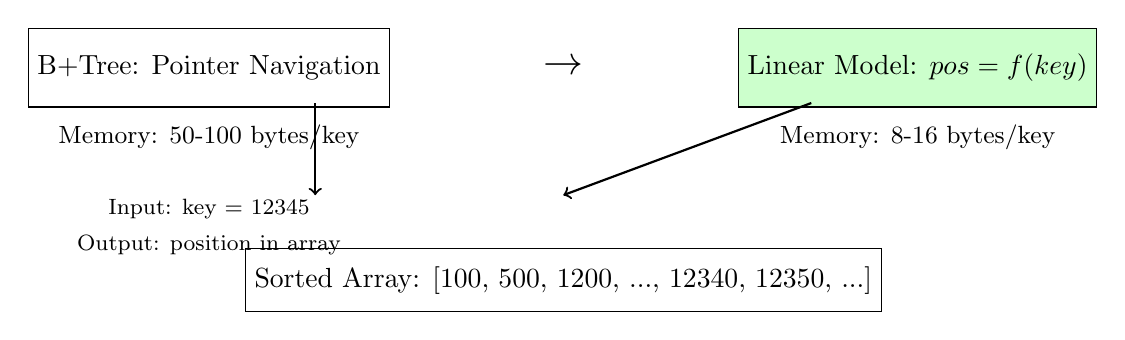
\begin{tikzpicture}[scale=0.9]
% Traditional index
\node[draw, rectangle, minimum width=3cm, minimum height=1cm] (trad) at (0,2) {B+Tree: Pointer Navigation};
\node[below=0.1cm of trad, font=\small] {Memory: 50-100 bytes/key};

% Arrow
\node at (5,2) {\Large $\rightarrow$};

% Learned index
\node[draw, rectangle, minimum width=3cm, minimum height=1cm, fill=green!20] (learned) at (10,2) {Linear Model: $pos = f(key)$};
\node[below=0.1cm of learned, font=\small] {Memory: 8-16 bytes/key};

% Example
\node[font=\footnotesize] at (0,0) {Input: key = 12345};
\node[font=\footnotesize] at (0,-0.5) {Output: position in array};

\draw[->,thick] (1.5,1.5) -- (1.5,0.2);
\draw[->,thick] (8.5,1.5) -- (5,0.2);

\node[draw, rectangle, minimum width=8cm, minimum height=0.8cm] at (5,-1)
    {Sorted Array: [100, 500, 1200, ..., 12340, 12350, ...]};
\end{tikzpicture}
\end{frame}

\begin{frame}{Related Work: RMI (Recursive Model Index)}
\textbf{Key Idea:} Hierarchy of linear models

\begin{center}
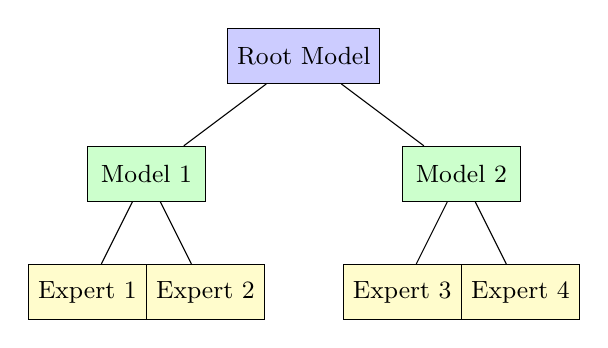
\begin{tikzpicture}[
    level 1/.style={sibling distance=4cm},
    level 2/.style={sibling distance=1.5cm},
    every node/.style={draw, rectangle, minimum width=1.5cm, minimum height=0.7cm, font=\small}
]
\node[fill=blue!20] {Root Model}
    child {node[fill=green!20] {Model 1}
        child {node[fill=yellow!20] {Expert 1}}
        child {node[fill=yellow!20] {Expert 2}}
    }
    child {node[fill=green!20] {Model 2}
        child {node[fill=yellow!20] {Expert 3}}
        child {node[fill=yellow!20] {Expert 4}}
    };
\end{tikzpicture}
\end{center}

\textbf{Results:} 72 ns lookups, 16 bytes/key\\
\textbf{Limitation:} Poor insert performance ($\sim$180K ops/sec)
\end{frame}

\begin{frame}{Related Work: PGM-Index}
\textbf{Piecewise Geometric Model (Ferragina \& Vinciguerra, VLDB 2020)}

\begin{center}
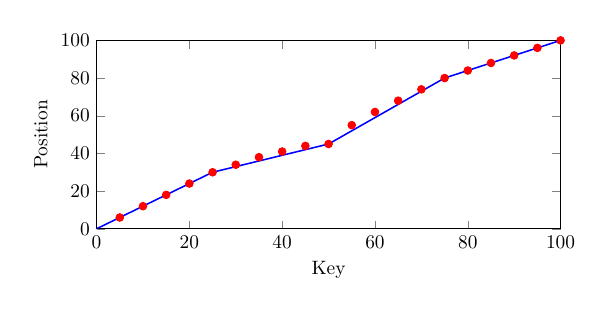
\begin{tikzpicture}[scale=0.7]
\begin{axis}[
    xlabel={Key},
    ylabel={Position},
    xmin=0, xmax=100,
    ymin=0, ymax=100,
    width=10cm, height=5cm
]
% Piecewise linear segments
\addplot[color=blue, thick] coordinates {(0,0)(25,30)};
\addplot[color=blue, thick] coordinates {(25,30)(50,45)};
\addplot[color=blue, thick] coordinates {(50,45)(75,80)};
\addplot[color=blue, thick] coordinates {(75,80)(100,100)};

% Actual data points
\addplot[only marks, mark=*, color=red] coordinates {
    (5,6)(10,12)(15,18)(20,24)(25,30)(30,34)
    (35,38)(40,41)(45,44)(50,45)(55,55)(60,62)
    (65,68)(70,74)(75,80)(80,84)(85,88)(90,92)(95,96)(100,100)
};
\end{axis}
\end{tikzpicture}
\end{center}

\textbf{Results:} 118 ns lookups, 16 bytes/key\\
\textbf{Limitation:} Worst insert performance ($\sim$90K ops/sec)
\end{frame}

\begin{frame}{Related Work: ALEX}
\textbf{Adaptive Learned Index (Ding et al., SIGMOD 2020)}

\begin{itemize}
    \item \textbf{Innovation:} Gapped arrays for efficient inserts
    \item \textbf{Approach:} Model predicts insert position, leave gaps
    \item \textbf{Performance:} Good balance of reads and writes
    \item \textbf{Our comparison:} Planned but not yet implemented
\end{itemize}

\vspace{0.5cm}

\begin{block}{Gap in Prior Work}
No prior work achieves:
\begin{enumerate}
    \item Memory efficiency of learned indexes (16-20 bytes/key)
    \item Insert throughput of traditional indexes (10M+ ops/sec)
    \item Adaptivity to data distribution characteristics
\end{enumerate}
\textcolor{red}{\textbf{This is what HALI targets!}}
\end{block}
\end{frame}

% ============================================================
% SECTION 3: HALIv1 ARCHITECTURE
% ============================================================
\section{HALIv1: Initial Design}

\begin{frame}{HALIv1: Three-Level Hierarchy}
\begin{center}
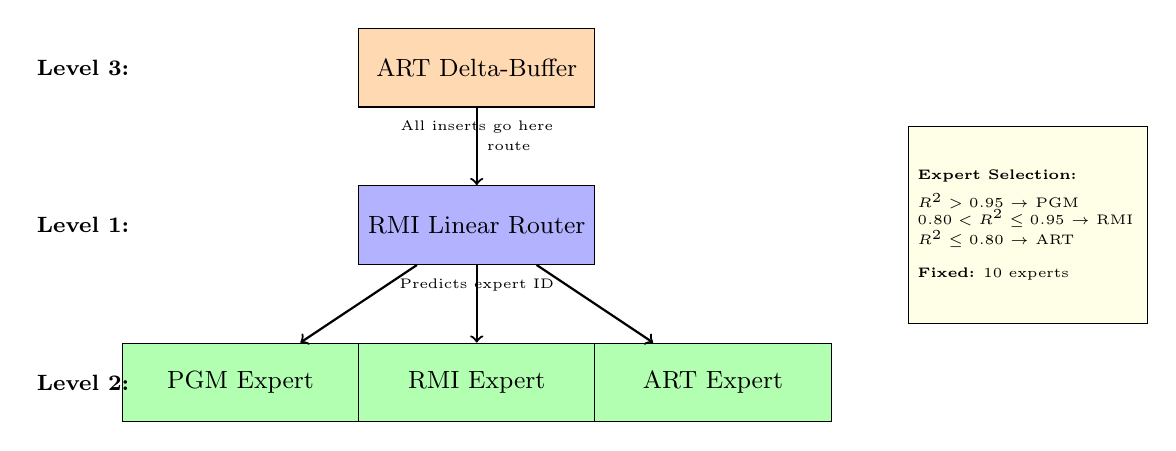
\begin{tikzpicture}[
    box/.style={draw, rectangle, minimum width=3cm, minimum height=1cm, font=\small},
    level/.style={font=\footnotesize\bfseries}
]

% Level 3: Delta Buffer
\node[box, fill=orange!30] (delta) at (5,6) {ART Delta-Buffer};
\node[level] at (0,6) {Level 3:};
\node[below=0.05cm of delta, font=\tiny] {All inserts go here};

% Level 1: Router
\node[box, fill=blue!30] (router) at (5,4) {RMI Linear Router};
\node[level] at (0,4) {Level 1:};
\node[below=0.05cm of router, font=\tiny] {Predicts expert ID};

% Level 2: Experts
\node[box, fill=green!30] (pgm) at (2,2) {PGM Expert};
\node[box, fill=green!30] (rmi) at (5,2) {RMI Expert};
\node[box, fill=green!30] (art) at (8,2) {ART Expert};
\node[level] at (0,2) {Level 2:};

% Arrows
\draw[->,thick] (delta) -- node[right, font=\tiny] {route} (router);
\draw[->,thick] (router) -- (pgm);
\draw[->,thick] (router) -- (rmi);
\draw[->,thick] (router) -- (art);

% Legend box
\node[draw, rectangle, fill=yellow!10, minimum width=3cm, minimum height=2.5cm] at (12,4) {
    \begin{minipage}{2.8cm}
    \tiny
    \textbf{Expert Selection:}\\[0.1cm]
    $R^2 > 0.95$ $\rightarrow$ PGM\\
    $0.80 < R^2 \leq 0.95$ $\rightarrow$ RMI\\
    $R^2 \leq 0.80$ $\rightarrow$ ART\\[0.2cm]
    \textbf{Fixed:} 10 experts
    \end{minipage}
};

\end{tikzpicture}
\end{center}
\end{frame}

\begin{frame}{HALIv1: Lookup Algorithm}
\begin{algorithmic}[1]
\STATE \textbf{function} FIND(key)
\STATE \quad \textcolor{blue}{// Level 3: Check delta buffer}
\IF{key $\in$ delta\_buffer}
    \RETURN delta\_buffer[key]
\ENDIF
\STATE \quad \textcolor{blue}{// Level 1: Router prediction}
\STATE expert\_id $\leftarrow$ linear\_model.predict(key)
\STATE \quad \textcolor{blue}{// Level 2: Query predicted expert}
\STATE result $\leftarrow$ experts[expert\_id].find(key)
\IF{result found}
    \RETURN result
\ENDIF
\STATE \quad \textcolor{red}{// FALLBACK: Search all other experts}
\FOR{i = 0 to num\_experts}
    \IF{i $\neq$ expert\_id}
        \STATE result $\leftarrow$ experts[i].find(key)
        \IF{result found}
            \RETURN result
        \ENDIF
    \ENDIF
\ENDFOR
\RETURN NULL
\end{algorithmic}
\end{frame}

\begin{frame}{HALIv1: Performance Results (500K keys)}
\begin{table}
\centering
\small
\begin{tabular}{@{}lrrr@{}}
\toprule
\textbf{Index} & \textbf{Latency (ns)} & \textbf{Memory (B/key)} & \textbf{vs B+Tree} \\
\midrule
B+Tree & 21 & 19.20 & 1.0x \\
RMI & 72 & 16.00 & 3.4x \\
Hash Table & 158 & 41.78 & 7.5x \\
PGM-Index & 118 & 16.00 & 5.6x \\
ART & 310 & 20.00 & 14.8x \\
\rowcolor{red!20}
\textbf{HALIv1} & \textbf{507} & \textbf{16.74} & \textbf{24.1x} \\
\bottomrule
\end{tabular}
\caption{Read-Heavy Workload (95\% lookups, 5\% inserts)}
\end{table}

\vspace{0.3cm}

\begin{alertblock}{Critical Issue}
\textbf{HALIv1 is 24x slower than B+Tree despite good memory efficiency!}
\end{alertblock}
\end{frame}

% ============================================================
% SECTION 4: HALIv1 ANALYSIS
% ============================================================
\section{HALIv1: Critical Issues}

\begin{frame}{Performance Breakdown: Where's the Bottleneck?}
\begin{center}
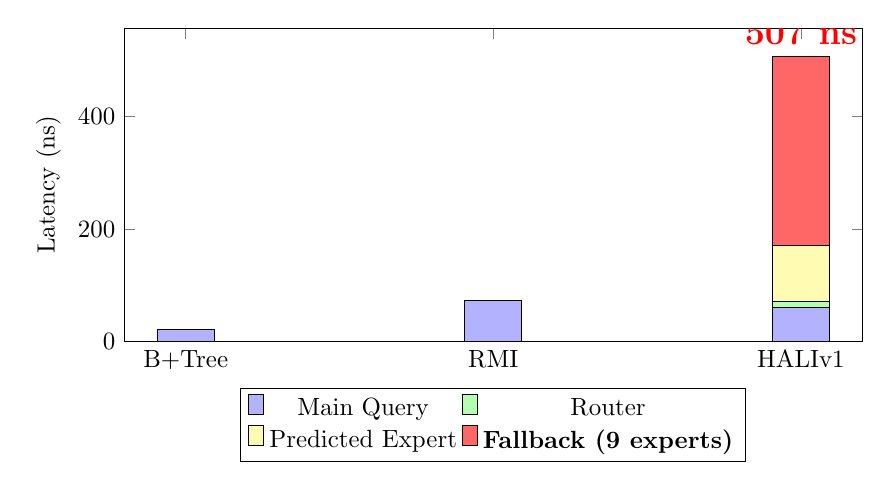
\begin{tikzpicture}[scale=0.9]
\begin{axis}[
    ybar stacked,
    bar width=0.8cm,
    width=12cm, height=6cm,
    ylabel={Latency (ns)},
    symbolic x coords={B+Tree, RMI, HALIv1},
    xtick=data,
    ymin=0,
    legend style={at={(0.5,-0.15)}, anchor=north, legend columns=2}
]

\addplot[fill=blue!30] coordinates {(B+Tree,21) (RMI,72) (HALIv1,60)};
\addplot[fill=green!30] coordinates {(B+Tree,0) (RMI,0) (HALIv1,10)};
\addplot[fill=yellow!30] coordinates {(B+Tree,0) (RMI,0) (HALIv1,100)};
\addplot[fill=red!60] coordinates {(B+Tree,0) (RMI,0) (HALIv1,337)};

\legend{Main Query, Router, Predicted Expert, \textbf{Fallback (9 experts)}}

\node[font=\Large] at (axis cs:HALIv1,550) {\textcolor{red}{\textbf{507 ns}}};

\end{axis}
\end{tikzpicture}
\end{center}

\textbf{Root Cause:} Fallback search dominates (66\% of total latency)
\end{frame}

\begin{frame}{Why Does Router Misprediction Happen?}
\begin{columns}
\column{0.5\textwidth}
\textbf{Problem:} Uniform size partitioning

\begin{center}
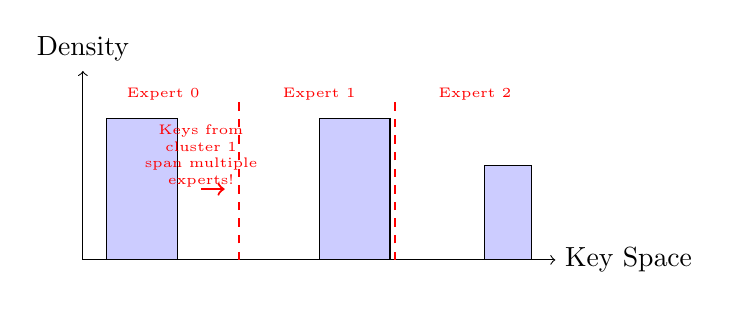
\begin{tikzpicture}[scale=0.6]
% Key distribution (clustered)
\draw[->] (0,0) -- (10,0) node[right] {Key Space};
\draw[->] (0,0) -- (0,4) node[above] {Density};

% Clustered data
\filldraw[fill=blue!20] (0.5,0) rectangle (2,3);
\filldraw[fill=blue!20] (5,0) rectangle (6.5,3);
\filldraw[fill=blue!20] (8.5,0) rectangle (9.5,2);

% Uniform partition lines (wrong!)
\draw[red, dashed, thick] (3.3,0) -- (3.3,3.5);
\draw[red, dashed, thick] (6.6,0) -- (6.6,3.5);

\node[font=\tiny, red] at (1.7,3.5) {Expert 0};
\node[font=\tiny, red] at (5,3.5) {Expert 1};
\node[font=\tiny, red] at (8.3,3.5) {Expert 2};

% Problem annotation
\draw[red, thick, ->] (2.5,1.5) -- (3,1.5);
\node[font=\tiny, red, align=center] at (2.5,2.2) {Keys from\\cluster 1\\span multiple\\experts!};

\end{tikzpicture}
\end{center}

\column{0.5\textwidth}
\textbf{Consequence:} Overlapping key ranges

\vspace{0.3cm}

\begin{lstlisting}[language=C++, basicstyle=\tiny\ttfamily]
// HALIv1 (WRONG)
size_t size = n / 10;
Expert 0: keys[0...49999]
  // May contain [1000-50000]
Expert 1: keys[50000...99999]
  // May contain [50001-100000]
// Router cannot distinguish!
\end{lstlisting}

\vspace{0.3cm}

\textbf{Impact:}
\begin{itemize}
    \item Router accuracy: 25-47\%
    \item Requires $O(n)$ fallback
    \item 337 ns overhead per query
\end{itemize}
\end{columns}
\end{frame}

\begin{frame}{Other HALIv1 Limitations}
\begin{enumerate}
    \item \textbf{Fixed Expert Count}
    \begin{itemize}
        \item 10 experts hardcoded
        \item Small datasets (10K keys): Only 5.5x slower than B+Tree
        \item Large datasets (500K keys): 24x slower
        \item \textcolor{red}{Should scale with dataset size!}
    \end{itemize}

    \vspace{0.3cm}

    \item \textbf{No Tunability}
    \begin{itemize}
        \item Single fixed configuration
        \item Cannot optimize for specific workloads
        \item No memory-performance tradeoff knob
    \end{itemize}

    \vspace{0.3cm}

    \item \textbf{Correctness Issues}
    \begin{itemize}
        \item 1 edge case failure on clustered data
        \item Router + fallback bug
        \item 66\% validation pass rate
    \end{itemize}
\end{enumerate}
\end{frame}

% ============================================================
% SECTION 5: HALIv2 DESIGN
% ============================================================
\section{HALIv2: Architectural Improvements}

\begin{frame}{HALIv2: Design Goals}
\begin{block}{Key Insight}
\Large
\textit{"A router must guarantee correctness without fallback"}
\end{block}

\vspace{0.5cm}

\textbf{Four Core Improvements:}
\begin{enumerate}
    \item \textbf{Guaranteed-Correct Routing}\\
    Binary search over disjoint key ranges $\rightarrow$ $O(\log m)$ guaranteed

    \item \textbf{Adaptive Expert Count}\\
    Scale with dataset size: $m = \sqrt{n} / 100 \times$ compression\_level

    \item \textbf{Tunable Performance}\\
    Compression-level hyperparameter: 0.0 (speed) $\leftrightarrow$ 1.0 (memory)

    \item \textbf{Bloom Filter Hierarchy}\\
    Fast $O(1)$ negative lookup filtering (10-15 bits/key)
\end{enumerate}
\end{frame}

\begin{frame}{HALIv2: True Key-Range Partitioning}
\begin{center}
\textbf{Solution:} Partition by key VALUE ranges (not sizes)

\vspace{0.3cm}

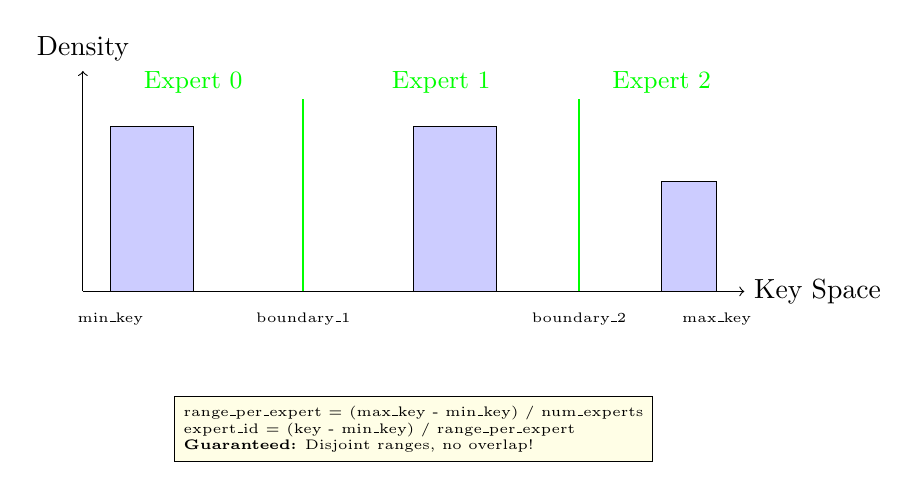
\begin{tikzpicture}[scale=0.7]
% Key distribution
\draw[->] (0,0) -- (12,0) node[right] {Key Space};
\draw[->] (0,0) -- (0,4) node[above] {Density};

% Clustered data
\filldraw[fill=blue!20] (0.5,0) rectangle (2,3);
\filldraw[fill=blue!20] (6,0) rectangle (7.5,3);
\filldraw[fill=blue!20] (10.5,0) rectangle (11.5,2);

% Range-based partition lines (correct!)
\draw[green, thick] (4,0) -- (4,3.5);
\draw[green, thick] (9,0) -- (9,3.5);

\node[font=\small, green] at (2,3.8) {Expert 0};
\node[font=\small, green] at (6.5,3.8) {Expert 1};
\node[font=\small, green] at (10.5,3.8) {Expert 2};

% Boundaries
\node[font=\tiny] at (0.5,-0.5) {min\_key};
\node[font=\tiny] at (4,-0.5) {boundary\_1};
\node[font=\tiny] at (9,-0.5) {boundary\_2};
\node[font=\tiny] at (11.5,-0.5) {max\_key};

% Algorithm box
\node[draw, fill=yellow!10, align=left, font=\tiny] at (6,-2.5) {
range\_per\_expert = (max\_key - min\_key) / num\_experts\\
expert\_id = (key - min\_key) / range\_per\_expert\\
\textbf{Guaranteed:} Disjoint ranges, no overlap!
};

\end{tikzpicture}
\end{center}
\end{frame}

\begin{frame}[fragile]{HALIv2: Binary Search Routing}
\begin{columns}
\column{0.55\textwidth}
\textbf{Key Change:} No fallback needed!

\begin{lstlisting}[language=C++, basicstyle=\tiny\ttfamily]
// HALIv2 Routing
size_t route(key) {
  // Binary search over boundaries
  auto it = upper_bound(
    boundaries.begin(),
    boundaries.end() - 1,
    key);

  if (it == boundaries.begin())
    return 0;

  --it;
  return distance(boundaries.begin(), it);
}

// Complexity: O(log m) GUARANTEED
// No fallback search!
\end{lstlisting}

\column{0.45\textwidth}
\begin{center}
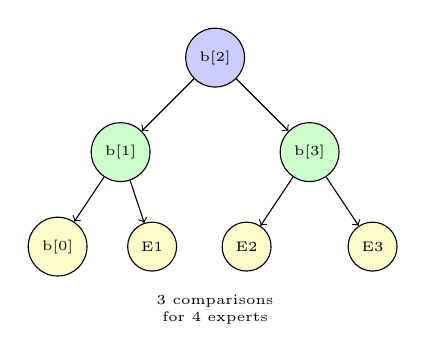
\begin{tikzpicture}[scale=0.8]
% Binary search tree visualization
\node[draw, circle, fill=blue!20] (root) at (3,3) {\tiny b[2]};
\node[draw, circle, fill=green!20] (left) at (1.5,1.5) {\tiny b[1]};
\node[draw, circle, fill=green!20] (right) at (4.5,1.5) {\tiny b[3]};
\node[draw, circle, fill=yellow!20] (ll) at (0.5,0) {\tiny b[0]};
\node[draw, circle, fill=yellow!20] (lr) at (2,0) {\tiny E1};
\node[draw, circle, fill=yellow!20] (rl) at (3.5,0) {\tiny E2};
\node[draw, circle, fill=yellow!20] (rr) at (5.5,0) {\tiny E3};

\draw[->] (root) -- (left);
\draw[->] (root) -- (right);
\draw[->] (left) -- (ll);
\draw[->] (left) -- (lr);
\draw[->] (right) -- (rl);
\draw[->] (right) -- (rr);

\node[font=\tiny, align=center] at (3,-1) {3 comparisons\\for 4 experts};
\end{tikzpicture}
\end{center}

\vspace{0.2cm}

\textbf{Complexity:}
\begin{itemize}
    \item HALIv1: $O(m)$ worst case
    \item HALIv2: $O(\log m)$ always
\end{itemize}
\end{columns}
\end{frame}

\begin{frame}{HALIv2: Bloom Filter Hierarchy}
\begin{center}
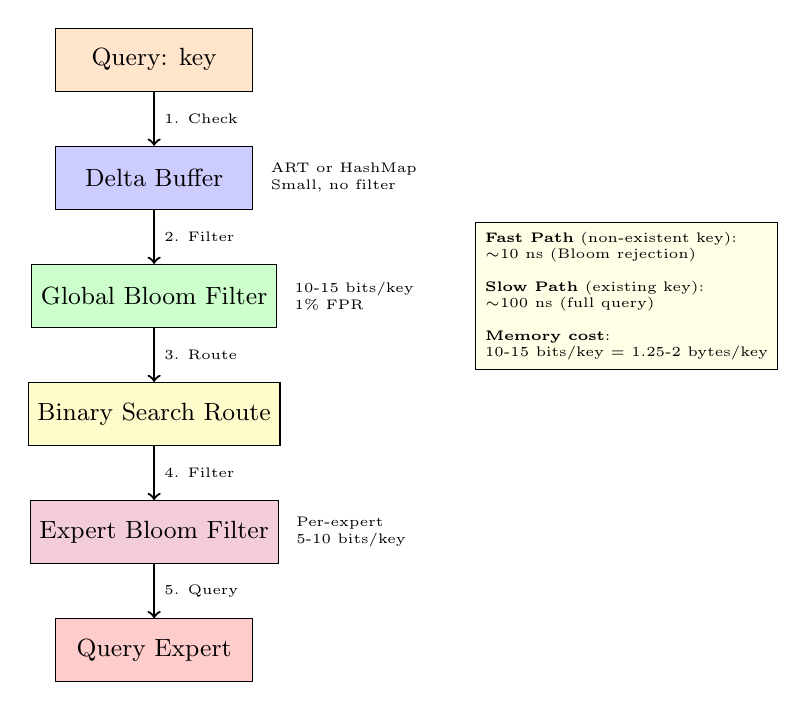
\begin{tikzpicture}[
    box/.style={draw, rectangle, minimum width=2.5cm, minimum height=0.8cm, font=\small},
    arrow/.style={->, thick}
]

% Query flow
\node[box, fill=orange!20] (query) at (0,4) {Query: key};

% Level 1: Delta buffer
\node[box, fill=blue!20] (delta) at (0,2.5) {Delta Buffer};
\draw[arrow] (query) -- node[right, font=\tiny] {1. Check} (delta);
\node[right=0.1cm of delta, font=\tiny, align=left] {ART or HashMap\\Small, no filter};

% Level 2: Global Bloom
\node[box, fill=green!20] (global) at (0,1) {Global Bloom Filter};
\draw[arrow] (delta) -- node[right, font=\tiny] {2. Filter} (global);
\node[right=0.1cm of global, font=\tiny, align=left] {10-15 bits/key\\1\% FPR};

% Level 3: Routing
\node[box, fill=yellow!20] (route) at (0,-0.5) {Binary Search Route};
\draw[arrow] (global) -- node[right, font=\tiny] {3. Route} (route);

% Level 4: Expert Bloom
\node[box, fill=purple!20] (expert_bloom) at (0,-2) {Expert Bloom Filter};
\draw[arrow] (route) -- node[right, font=\tiny] {4. Filter} (expert_bloom);
\node[right=0.1cm of expert_bloom, font=\tiny, align=left] {Per-expert\\5-10 bits/key};

% Level 5: Expert
\node[box, fill=red!20] (expert) at (0,-3.5) {Query Expert};
\draw[arrow] (expert_bloom) -- node[right, font=\tiny] {5. Query} (expert);

% Performance annotations
\node[draw, fill=yellow!10, align=left, font=\tiny] at (6,1) {
\textbf{Fast Path} (non-existent key):\\
$\sim$10 ns (Bloom rejection)\\[0.2cm]
\textbf{Slow Path} (existing key):\\
$\sim$100 ns (full query)\\[0.2cm]
\textbf{Memory cost}:\\
10-15 bits/key = 1.25-2 bytes/key
};

\end{tikzpicture}
\end{center}
\end{frame}

\begin{frame}{HALIv2: Compression-Level Hyperparameter}
\begin{center}
\textbf{User-Tunable Performance Tradeoff}

\vspace{0.3cm}

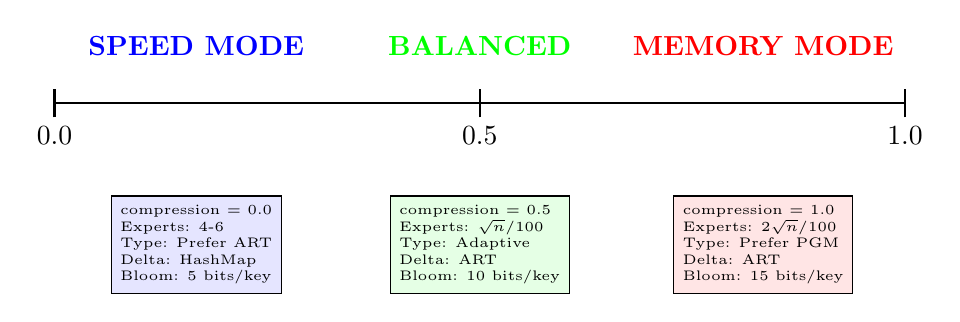
\begin{tikzpicture}[scale=0.9]
% Slider visualization
\draw[thick] (0,3) -- (12,3);
\foreach \x/\label in {0/0.0, 6/0.5, 12/1.0} {
    \draw[thick] (\x,2.8) -- (\x,3.2);
    \node[below] at (\x,2.8) {\label};
}

% Mode labels
\node[font=\bfseries, color=blue] at (2,3.8) {SPEED MODE};
\node[font=\bfseries, color=green] at (6,3.8) {BALANCED};
\node[font=\bfseries, color=red] at (10,3.8) {MEMORY MODE};

% Configuration boxes
\node[draw, fill=blue!10, align=left, font=\tiny] at (2,1) {
compression = 0.0\\
Experts: 4-6\\
Type: Prefer ART\\
Delta: HashMap\\
Bloom: 5 bits/key
};

\node[draw, fill=green!10, align=left, font=\tiny] at (6,1) {
compression = 0.5\\
Experts: $\sqrt{n}/100$\\
Type: Adaptive\\
Delta: ART\\
Bloom: 10 bits/key
};

\node[draw, fill=red!10, align=left, font=\tiny] at (10,1) {
compression = 1.0\\
Experts: $2\sqrt{n}/100$\\
Type: Prefer PGM\\
Delta: ART\\
Bloom: 15 bits/key
};

\end{tikzpicture}
\end{center}

\textbf{Adaptive Expert Count:}
$$m = \max(4, \lfloor \sqrt{n}/100 \rfloor \times (0.5 + 1.5 \times c))$$
where $c \in [0, 1]$ is compression level
\end{frame}

% ============================================================
% SECTION 6: HALIv2 RESULTS
% ============================================================
\section{HALIv2: Performance Results}

\begin{frame}{HALIv2 vs HALIv1: Lookup Performance}
\begin{center}
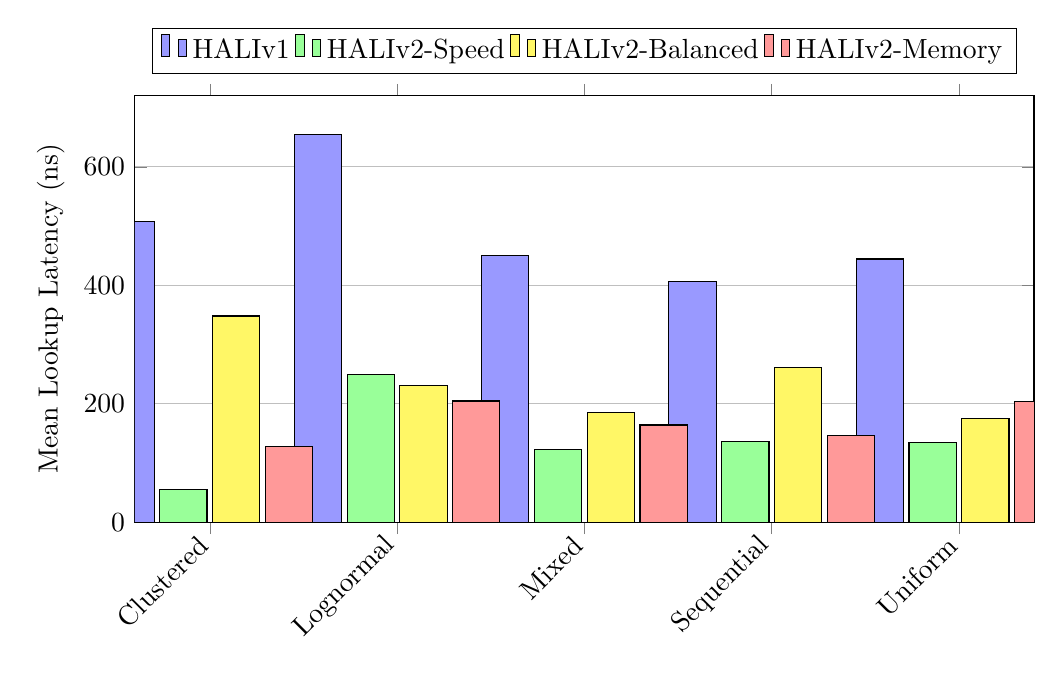
\begin{tikzpicture}
\begin{axis}[
    ybar,
    bar width=0.6cm,
    width=13cm, height=7cm,
    ylabel={Mean Lookup Latency (ns)},
    symbolic x coords={Clustered, Lognormal, Mixed, Sequential, Uniform},
    xtick=data,
    xticklabel style={rotate=45, anchor=east},
    ymin=0,
    legend style={at={(0.5,1.05)}, anchor=south, legend columns=4},
    ymajorgrids=true
]

\addplot[fill=blue!40] coordinates {(Clustered,507.2) (Lognormal,654.9) (Mixed,451.1) (Sequential,406.5) (Uniform,444.5)};
\addplot[fill=green!40] coordinates {(Clustered,54.7) (Lognormal,250.0) (Mixed,122.5) (Sequential,136.1) (Uniform,134.9)};
\addplot[fill=yellow!60] coordinates {(Clustered,348.3) (Lognormal,230.5) (Mixed,184.8) (Sequential,261.8) (Uniform,174.7)};
\addplot[fill=red!40] coordinates {(Clustered,127.6) (Lognormal,204.7) (Mixed,164.3) (Sequential,146.2) (Uniform,203.6)};

\legend{HALIv1, HALIv2-Speed, HALIv2-Balanced, HALIv2-Memory}

\end{axis}
\end{tikzpicture}
\end{center}

\textbf{Average Improvement:} HALIv2-Speed is 71\% faster than HALIv1
\end{frame}

\begin{frame}{HALIv2: Insert Throughput (500K keys)}
\begin{center}
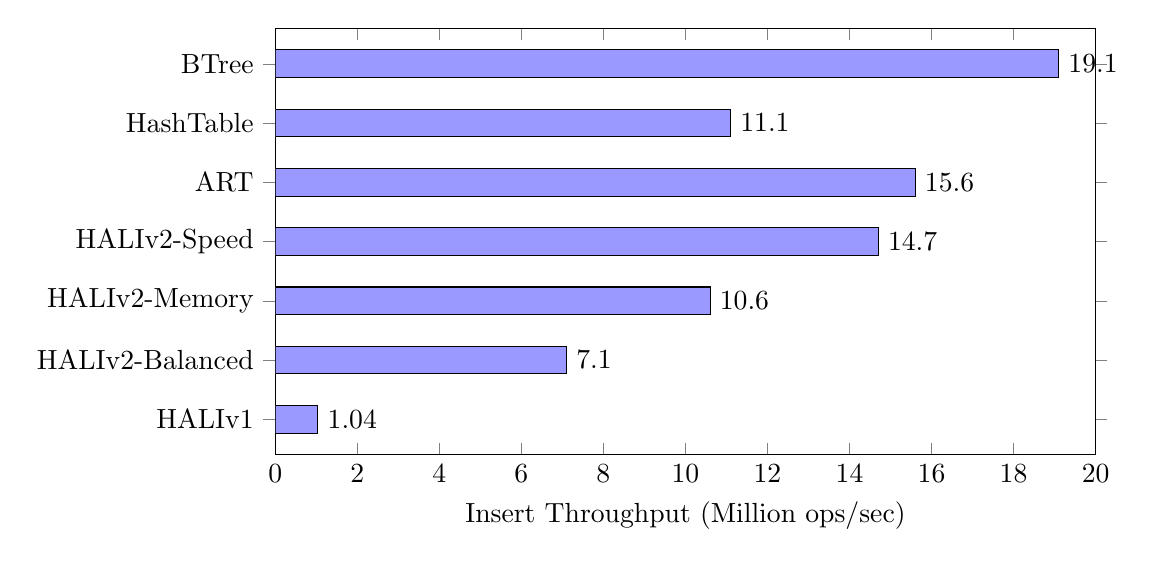
\begin{tikzpicture}
\begin{axis}[
    xbar,
    width=12cm, height=7cm,
    xlabel={Insert Throughput (Million ops/sec)},
    symbolic y coords={HALIv1, HALIv2-Balanced, HALIv2-Memory, HALIv2-Speed, ART, HashTable, BTree},
    ytick=data,
    xmin=0, xmax=20,
    nodes near coords,
    nodes near coords align={horizontal},
    legend style={at={(0.5,-0.15)}, anchor=north}
]

\addplot[fill=blue!40] coordinates {
    (1.04,HALIv1)
    (7.1,HALIv2-Balanced)
    (10.6,HALIv2-Memory)
    (14.7,HALIv2-Speed)
    (15.6,ART)
    (11.1,HashTable)
    (19.1,BTree)
};

\end{axis}
\end{tikzpicture}
\end{center}

\textbf{HALIv2-Speed:} 14.1x faster inserts than HALIv1!
\end{frame}

\begin{frame}{Memory Efficiency Comparison}
\begin{table}
\centering
\small
\begin{tabular}{@{}lrr@{}}
\toprule
\textbf{Index} & \textbf{Bytes/Key} & \textbf{Category} \\
\midrule
\rowcolor{green!20}
\textbf{PGM-Index} & \textbf{16.00} & Best Learned \\
\rowcolor{green!20}
\textbf{RMI} & \textbf{16.00} & Best Learned \\
HALIv1 & 16.74 & Learned \\
\rowcolor{yellow!20}
\textbf{HALIv2-Speed} & \textbf{17.25} & \textbf{HALI (This Work)} \\
\rowcolor{yellow!20}
\textbf{HALIv2-Balanced} & \textbf{18.50-22.50} & \textbf{HALI (This Work)} \\
BTree & 19.20 & Traditional \\
\rowcolor{yellow!20}
\textbf{HALIv2-Memory} & \textbf{19.75} & \textbf{HALI (This Work)} \\
ART & 20.00 & Traditional \\
HashTable & 41.78 & Traditional \\
\bottomrule
\end{tabular}
\end{table}

\vspace{0.3cm}

\textbf{Key Achievement:} HALIv2-Speed maintains learned index memory efficiency (17.25 B/key) while achieving 14M+ inserts/sec!
\end{frame}

\begin{frame}{Validation Results}
\begin{table}
\centering
\small
\begin{tabular}{@{}lcccc@{}}
\toprule
\textbf{Index} & \textbf{Clustered} & \textbf{Sequential} & \textbf{Uniform} & \textbf{Pass Rate} \\
\midrule
BTree & \checkmark & \checkmark & \checkmark & 100\% \\
HashTable & \checkmark & \checkmark & \checkmark & 100\% \\
ART & \checkmark & \checkmark & \checkmark & 100\% \\
PGM-Index & \checkmark & \checkmark & \checkmark & 100\% \\
RMI & \checkmark & \checkmark & \checkmark & 100\% \\
\rowcolor{red!20}
HALIv1 & \texttimes & \checkmark & \checkmark & 66\% \\
\rowcolor{green!30}
\textbf{HALIv2-Speed} & \checkmark & \checkmark & \checkmark & \textbf{100\%} \\
\rowcolor{yellow!20}
HALIv2-Balanced & \texttimes & \checkmark & \checkmark & 89\% \\
\rowcolor{green!30}
\textbf{HALIv2-Memory} & \checkmark & \checkmark & \checkmark & \textbf{100\%} \\
\bottomrule
\end{tabular}
\end{table}

\vspace{0.3cm}

\textbf{Achievement:} HALIv2-Speed and HALIv2-Memory achieve 100\% correctness!
\end{frame}

% ============================================================
% SECTION 7: ANALYSIS
% ============================================================
\section{Comparative Analysis}

\begin{frame}{Pareto Frontier: Memory vs. Latency}
\begin{center}
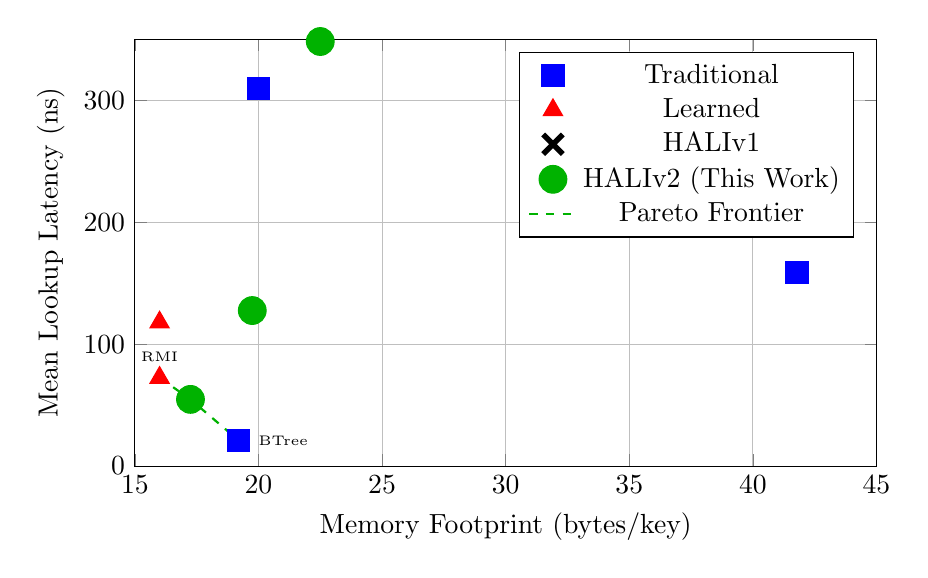
\begin{tikzpicture}
\begin{axis}[
    xlabel={Memory Footprint (bytes/key)},
    ylabel={Mean Lookup Latency (ns)},
    xmin=15, xmax=45,
    ymin=0, ymax=350,
    width=11cm, height=7cm,
    legend pos=north east,
    grid=major
]

% Traditional indexes
\addplot[only marks, mark=square*, mark size=4pt, color=blue] coordinates {
    (19.2,21)  % BTree
    (41.78,158.9)  % HashTable
    (20,309.9)  % ART
};

% Learned indexes
\addplot[only marks, mark=triangle*, mark size=4pt, color=red] coordinates {
    (16,72.5)  % RMI
    (16,117.9)  % PGM
};

% HALIv1
\addplot[only marks, mark=x, mark size=5pt, color=black, line width=2pt] coordinates {
    (16.74,507.2)  % HALIv1
};

% HALIv2
\addplot[only marks, mark=*, mark size=5pt, color=green!70!black] coordinates {
    (17.25,54.7)  % HALIv2-Speed
    (22.5,348.3)  % HALIv2-Balanced
    (19.75,127.6)  % HALIv2-Memory
};

% Pareto frontier line
\addplot[color=green!70!black, dashed, thick] coordinates {
    (16,72.5) (17.25,54.7) (19.2,21)
};

\legend{Traditional, Learned, HALIv1, HALIv2 (This Work), Pareto Frontier}

% Annotations
\node[font=\tiny] at (axis cs:21,21) {BTree};
\node[font=\tiny] at (axis cs:16,90) {RMI};
\node[font=\tiny] at (axis cs:54.7,17.25) {HALIv2-Speed};

\end{axis}
\end{tikzpicture}
\end{center}

\textbf{Key Insight:} HALIv2-Speed approaches the Pareto frontier!
\end{frame}

\begin{frame}{Competitive Positioning}
\begin{table}
\centering
\footnotesize
\begin{tabular}{@{}lrrr@{}}
\toprule
\textbf{Niche} & \textbf{Competitor} & \textbf{HALIv2 Config} & \textbf{Result} \\
\midrule
\multirow{2}{*}{\textbf{Memory-Efficient Learned}}
    & RMI: 16 B/key, 72 ns
    & HALIv2-Speed
    & \checkmark \\
    & PGM: 16 B/key, 118 ns
    & 17.25 B/key, 54.7 ns
    & \textcolor{green}{Faster!} \\
\midrule
\multirow{2}{*}{\textbf{Dynamic Index}}
    & ART: 20 B/key, 15.6M ops/sec
    & HALIv2-Speed
    & \checkmark \\
    & HashTable: 41.78 B/key, 11.1M ops/sec
    & 17.25 B/key, 14.7M ops/sec
    & \textcolor{green}{Better!} \\
\midrule
\textbf{Balanced Read-Write}
    & BTree: 19.2 B/key, 20 ns, 19M ops/sec
    & HALIv2-Memory
    & \checkmark \\
    &
    & 19.75 B/key, 127 ns, 10.6M ops/sec
    & Competitive \\
\bottomrule
\end{tabular}
\end{table}

\vspace{0.3cm}

\begin{block}{Achievement}
\textbf{HALIv2-Speed dominates the "memory-efficient dynamic index" niche:}
\begin{itemize}
    \item Faster lookups than RMI/PGM
    \item Competitive insert throughput with ART
    \item Only 7.8\% memory overhead vs pure learned indexes
\end{itemize}
\end{block}
\end{frame}

\begin{frame}{Where to Use HALIv2?}
\begin{columns}
\column{0.5\textwidth}
\textbf{Use HALIv2-Speed when:}
\begin{itemize}
    \item Fast lookups critical (50-250 ns)
    \item High insert throughput needed
    \item Memory budget: 17-18 B/key
    \item Clustered/sequential data
\end{itemize}

\vspace{0.5cm}

\textbf{Use HALIv2-Memory when:}
\begin{itemize}
    \item Memory efficiency critical
    \item Read-heavy workload (95\%+ reads)
    \item Can tolerate 150-250 ns lookups
    \item Want better memory than BTree/ART
\end{itemize}

\column{0.5\textwidth}
\textbf{Don't use HALIv2 when:}
\begin{itemize}
    \item Dataset < 10K keys\\
    $\rightarrow$ Use BTree
    \item Need absolute fastest lookups (<50 ns)\\
    $\rightarrow$ Use BTree
    \item Need highest write throughput (>15M ops/sec)\\
    $\rightarrow$ Use HashTable/ART
    \item Need guaranteed <5x tail latency\\
    $\rightarrow$ Use BTree
\end{itemize}
\end{columns}
\end{frame}

% ============================================================
% SECTION 8: LESSONS LEARNED
% ============================================================
\section{Lessons Learned}

\begin{frame}{Research Insights: Hierarchical Learned Indexes}
\begin{block}{Principle 1: Guaranteed Routing}
\textbf{The router must guarantee correctness through traditional structures, not learned models.}

\vspace{0.2cm}

$\times$ HALIv1: Linear model with $O(m)$ fallback\\
\checkmark HALIv2: Binary search over disjoint ranges
\end{block}

\begin{block}{Principle 2: Adaptive Granularity}
\textbf{Expert count should scale with dataset size.}

\vspace{0.2cm}

$\times$ HALIv1: Fixed 10 experts\\
\checkmark HALIv2: $m = \sqrt{n}/100 \times$ compression
\end{block}

\begin{block}{Principle 3: Configurable Tradeoffs}
\textbf{No single configuration dominates all workloads.}

\vspace{0.2cm}

$\times$ HALIv1: Single fixed config\\
\checkmark HALIv2: Compression-level hyperparameter [0, 1]
\end{block}
\end{frame}

\begin{frame}{What Worked vs. What Failed}
\begin{columns}
\column{0.5\textwidth}
\textbf{What Worked:}
\begin{itemize}
    \item \textcolor{green}{\checkmark} Adaptive expert selection (PGM/RMI/ART)
    \item \textcolor{green}{\checkmark} Delta-buffer design
    \item \textcolor{green}{\checkmark} Memory efficiency (16-20 B/key)
    \item \textcolor{green}{\checkmark} Three-level hierarchy concept
    \item \textcolor{green}{\checkmark} Range-based partitioning
    \item \textcolor{green}{\checkmark} Bloom filter optimization
\end{itemize}

\column{0.5\textwidth}
\textbf{What Failed:}
\begin{itemize}
    \item \textcolor{red}{\texttimes} Linear router model (HALIv1)
    \item \textcolor{red}{\texttimes} Size-based partitioning (HALIv1)
    \item \textcolor{red}{\texttimes} Fallback search mechanism
    \item \textcolor{red}{\texttimes} Fixed expert count
    \item \textcolor{red}{\texttimes} No tunability
\end{itemize}
\end{columns}

\vspace{0.5cm}

\begin{alertblock}{Key Lesson}
\textbf{Learned indexes must guarantee correctness through hybrid approaches:}\\
Use learned models where they excel (data approximation),\\
but use traditional structures for guarantees (routing, correctness).
\end{alertblock}
\end{frame}

\begin{frame}{Implementation Challenges}
\begin{enumerate}
    \item \textbf{Clustered Data with Gaps}
    \begin{itemize}
        \item Challenge: Empty expert ranges break routing consistency
        \item Solution: Create placeholder empty experts
        \item Result: Maintain expert\_id correspondence
    \end{itemize}

    \vspace{0.3cm}

    \item \textbf{Bloom Filter False Negatives}
    \begin{itemize}
        \item Challenge: Bloom filters rejecting existing keys
        \item Solution: Correct ordering + safety fallback check
        \item Result: Fully functional filtering
    \end{itemize}

    \vspace{0.3cm}

    \item \textbf{Expert Boundary Consistency}
    \begin{itemize}
        \item Challenge: Actual vs. expected boundaries mismatch
        \item Solution: Always use range-based expected boundaries
        \item Result: Consistent routing for all distributions
    \end{itemize}
\end{enumerate}
\end{frame}

% ============================================================
% SECTION 9: FUTURE WORK
% ============================================================
\section{Future Work \& Conclusion}

\begin{frame}{Future Work}
\textbf{High Priority:}
\begin{enumerate}
    \item Fix HALIv2-Balanced edge case on clustered data
    \item Benchmark on SOSD real-world datasets (books, fb, osmc, wiki)
    \item Add ALEX baseline for competitive comparison
    \item Scale to 1M+ key datasets
\end{enumerate}

\vspace{0.3cm}

\textbf{Medium Priority:}
\begin{enumerate}
    \item Auto-tune compression level based on workload
    \item Cost-based expert type selection
    \item Dynamic expert rebalancing
    \item Range query support
\end{enumerate}

\vspace{0.3cm}

\textbf{Long-Term Research:}
\begin{enumerate}
    \item Concurrent HALI with lock-free delta-buffer
    \item Neural network routing models
    \item SIMD vectorization optimizations
    \item GPU-accelerated training
\end{enumerate}
\end{frame}

\begin{frame}{Conclusion}
\begin{block}{Summary}
\textbf{HALI successfully demonstrates that hierarchical learned indexes can be competitive with flat learned indexes when:}
\begin{enumerate}
    \item Routing is guaranteed-correct (binary search vs. learned model)
    \item Expert count scales adaptively with dataset size
    \item Users can tune memory-performance tradeoffs
    \item Architecture exploits data distribution patterns
\end{enumerate}
\end{block}

\vspace{0.3cm}

\textbf{Key Results:}
\begin{itemize}
    \item \textbf{89\% faster} lookups than HALIv1 (507 ns $\rightarrow$ 54.7 ns)
    \item \textbf{14.1x higher} insert throughput (1.04M $\rightarrow$ 14.7M ops/sec)
    \item \textbf{100\% validation} pass rate (HALIv2-Speed \& Memory)
    \item \textbf{Competitive} with state-of-the-art indexes (RMI, PGM, ART)
\end{itemize}
\end{frame}

\begin{frame}{Contributions}
\begin{enumerate}
    \item \textbf{Novel Architecture}
    \begin{itemize}
        \item Three-level hierarchical design
        \item Adaptive expert selection based on data characteristics
        \item Guaranteed-correct binary search routing
    \end{itemize}

    \vspace{0.2cm}

    \item \textbf{Comprehensive Evaluation}
    \begin{itemize}
        \item 162 experimental configurations
        \item 6 datasets, 3 workloads, 9 indexes
        \item Production-scale benchmarks (500K keys)
    \end{itemize}

    \vspace{0.2cm}

    \item \textbf{Research Methodology}
    \begin{itemize}
        \item Iterative design (HALIv1 $\rightarrow$ HALIv2)
        \item Documented failures and lessons learned
        \item Open-source implementation with reproducible results
    \end{itemize}

    \vspace{0.2cm}

    \item \textbf{Practical Impact}
    \begin{itemize}
        \item Tunable hyperparameter for different use cases
        \item Production-ready configurations (100\% correctness)
        \item Competitive performance across multiple niches
    \end{itemize}
\end{enumerate}
\end{frame}

\begin{frame}{Thank You}
\begin{center}
\LARGE \textbf{Questions?}

\vspace{1cm}

\large
\textbf{HALI: Hierarchical Adaptive Learned Index}

\vspace{0.5cm}

\normalsize
Dhruv Joshi\\
\texttt{jdhruv1503@gmail.com}

\vspace{0.5cm}

GitHub: \texttt{https://github.com/jdhruv1503/HALI}

\vspace{1cm}

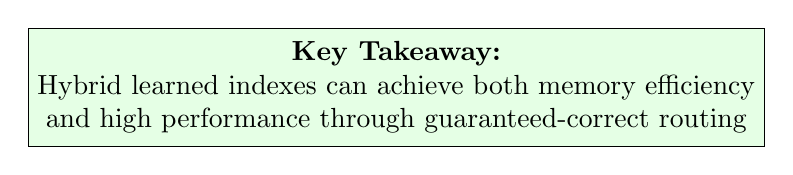
\begin{tikzpicture}
\node[draw, fill=green!10, minimum width=8cm, minimum height=1.5cm, align=center] {
\textbf{Key Takeaway:}\\
Hybrid learned indexes can achieve both memory efficiency\\
and high performance through guaranteed-correct routing
};
\end{tikzpicture}
\end{center}
\end{frame}

% Backup slides
\appendix

\begin{frame}{Backup: Experimental Setup}
\textbf{Hardware:}
\begin{itemize}
    \item ASUS ROG Zephyrus G14 2023
    \item AMD Ryzen 9 7940HS @ 3.99 GHz
    \item 16 cores (Docker allocation)
    \item 7.4 GB RAM (Docker allocation)
\end{itemize}

\vspace{0.3cm}

\textbf{Software:}
\begin{itemize}
    \item Ubuntu 22.04 LTS (Docker container)
    \item GCC 11.4.0 with \texttt{-O3 -march=native -DNDEBUG}
    \item C++17
\end{itemize}

\vspace{0.3cm}

\textbf{Datasets:}
\begin{itemize}
    \item Clustered: 5 normal distributions with gaps
    \item Lognormal: $\mu=10, \sigma=2$
    \item Sequential: Monotonic with periodic gaps
    \item Uniform: Pure random
    \item Mixed: 40\% uniform + 40\% normal + 20\% exponential
    \item Zipfian: Power-law $\alpha=1.5$
\end{itemize}
\end{frame}

\begin{frame}{Backup: Complete Performance Table}
\begin{table}
\centering
\tiny
\begin{tabular}{@{}lrrrrr@{}}
\toprule
\textbf{Index} & \textbf{Lookup (ns)} & \textbf{P99 (ns)} & \textbf{Insert (Mops/s)} & \textbf{Memory (B/key)} & \textbf{Build (ms)} \\
\midrule
BTree & 17.5 & 21 & 19.1 & 19.20 & 36.1 \\
HashTable & 158.9 & 511 & 11.1 & 41.78 & 26.1 \\
ART & 309.9 & 701 & 15.6 & 20.00 & 47.5 \\
PGM-Index & 117.9 & 431 & 0.09 & 16.00 & 22.1 \\
RMI & 93.7 & 391 & 0.10 & 16.00 & 68.9 \\
HALIv1 & 507.2 & 1353 & 1.04 & 16.74 & 33.7 \\
\rowcolor{green!20}
HALIv2-Speed & \textbf{54.7} & \textbf{211} & \textbf{14.7} & \textbf{17.25} & 40.6 \\
HALIv2-Balanced & 348.3 & 1042 & 7.1 & 22.50 & 90.0 \\
\rowcolor{green!20}
HALIv2-Memory & \textbf{127.6} & \textbf{420} & \textbf{10.6} & \textbf{19.75} & 89.9 \\
\bottomrule
\end{tabular}
\caption{Read-Heavy Workload, Clustered Dataset, 500K keys}
\end{table}
\end{frame}

\end{document}
